\chapter{Datenaugmentierung -- theoretische Grundlagen}
\label{kap:augtheorie}

Der Praxisteil dieser Arbeit steht und fällt mit der Augmentierung. Dieses
Kapitel entwickelt daher zunächst unabhängig vom konkreten Anwendungsfall, was
Augmentierung formal leistet (Abschnitt~\ref{sec:augformal}), über welche
Mechanismen sie wirkt (Abschnitt~\ref{sec:augmechanismen}), welche
Verfahrensklassen sich etabliert haben (Abschnitt~\ref{sec:augtaxonomie}), welche
Besonderheiten bei der Objektdetektion gelten
(Abschnitt~\ref{sec:augdetektion}) und wo die Grenzen des Verfahrens liegen
(Abschnitt~\ref{sec:auggrenzen}). Abschnitt~\ref{sec:augsynthese} behandelt den
Grenzfall, um den es hier geht: Augmentierung, die die Trainingsverteilung nicht
erweitert, sondern vollständig erzeugt. Aus diesem Kapitel werden am Ende sechs
Anforderungen abgeleitet, an denen sich die konkrete Pipeline in
Kapitel~\ref{kap:pipeline} messen lässt.

\section{Begriff und formale Einordnung}
\label{sec:augformal}

\absatz{Definition.} Datenaugmentierung bezeichnet die künstliche Vergrößerung
eines Trainingsdatensatzes durch Transformationen, die den semantischen Gehalt
der Beispiele -- und damit ihre Beschriftung -- erhalten
\parencite{shorten2019}. Formal sei
$D = \{(x_i, y_i)\}_{i=1}^{n}$ der Trainingsdatensatz, $\mathcal{T}$ eine Familie
von Transformationen mit einer Verteilung $p(t)$ über $\mathcal{T}$, und
$\tau_t$ die zu $t$ gehörende \emph{Labeltransformation}. Anstelle des
empirischen Risikos
\begin{equation}
\hat{R}(f) \;=\; \frac{1}{n}\sum_{i=1}^{n} L\big(f(x_i),\, y_i\big)
\label{eq:erm}
\end{equation}
minimiert das Training dann das \emph{augmentierte} Risiko
\begin{equation}
\hat{R}_{\text{aug}}(f) \;=\; \frac{1}{n}\sum_{i=1}^{n}
\mathbb{E}_{t \sim p(t)}\Big[ L\big(f(t(x_i)),\, \tau_t(y_i)\big) \Big].
\label{eq:erm-aug}
\end{equation}

Zwei Punkte an Gleichung~\eqref{eq:erm-aug} sind für das Weitere zentral. Erstens
tritt neben $t$ stets die Labeltransformation $\tau_t$ auf. Bei der
Bildklassifikation ist $\tau_t = \mathrm{id}$ -- eine gespiegelte Katze bleibt
eine Katze --, weshalb Augmentierung dort begrifflich mit
\enquote{label-erhaltend} gleichgesetzt wird. Bei der Objektdetektion ist
$\tau_t \neq \mathrm{id}$: Boxkoordinaten müssen mittransformiert werden, und
genau dabei entstehen die in Abschnitt~\ref{sec:augdetektion} behandelten Fehler.
Zweitens ist $p(t)$ ein Modellierungsgegenstand und keine Nebensache: Sie legt
fest, \emph{wie häufig} und \emph{wie stark} eine Transformation auftritt. Die
vollständige Dokumentation von $p(t)$ ist damit die Mindestanforderung an eine
reproduzierbare Augmentierung -- und der Grund, warum in
Kapitel~\ref{kap:pipeline} für jede Transformation nicht nur der
Parameterbereich, sondern auch der gemessene Ist-Anteil angegeben wird.

\absatz{Verhältnis zur Vicinal Risk Minimization.} Gleichung~\eqref{eq:erm-aug}
lässt sich auch so lesen, dass jeder Datenpunkt durch eine \emph{Umgebung}
(\enquote{vicinity}) ersetzt wird, über die das Risiko gemittelt wird.
\textcite{chapelle2001} formalisieren dies als Vicinal Risk Minimization: Statt
der empirischen Verteilung $\hat{P}(x,y) = \frac{1}{n}\sum_i
\delta(x-x_i)\delta(y-y_i)$ wird eine geglättete Verteilung
$\hat{P}_{\text{vic}}$ verwendet, deren Träger über die Datenpunkte hinausreicht.
Augmentierung ist damit die anwendungsspezifische Wahl dieser Umgebung: Sie
kodiert, welche Nachbarschaft eines Beispiels als \enquote{dasselbe Objekt} gilt.
Verfahren wie \emph{mixup} \parencite{zhang2018mixup} berufen sich explizit auf
diesen Rahmen.

\absatz{Verhältnis zum induktiven Bias der Architektur.}
Abschnitt~\ref{sec:prinzipien} hat gezeigt, dass die Faltungsarchitektur
Translationsäquivarianz \emph{strukturell} garantiert
(Gleichung~\eqref{eq:aequivarianz}). Für alle anderen erwünschten Invarianzen --
Rotation, Skalierung, Beleuchtung, Farbstich, Teilverdeckung -- gibt es in einem
gewöhnlichen CNN keine solche Garantie; sie müssen aus Daten gelernt werden.
Augmentierung ist genau das Werkzeug, mit dem diese Invarianzen auf der
\emph{Datenseite} statt auf der Architekturseite eingebracht werden. Die
Arbeitsteilung lässt sich damit so zusammenfassen:

\begin{itemize}
  \item \textbf{Architektur:} Lokalität, Stationarität, Translationsäquivarianz
  (Faltung), begrenzte Translationsinvarianz (Subsampling).
  \item \textbf{Augmentierung:} alle übrigen Invarianzen der konkreten Domäne --
  und nur diese; jede Invarianz, die in der Domäne \emph{nicht} gilt, darf nicht
  antrainiert werden.
\end{itemize}

Der zweite Halbsatz ist der wesentliche Entwurfsgrundsatz. Eine
Augmentierung, die eine in der Realität nicht vorhandene Invarianz erzwingt,
verschlechtert das Modell, weil sie diskriminative Information entfernt. Ein
Beispiel aus dem vorliegenden Fall: Volle Rotationsinvarianz ist bei einem
Rohrende korrekt, weil Kamerarollwinkel und Stapelausrichtung beliebig sind. Bei
einem Verkehrszeichen wäre sie falsch.

\section{Wirkmechanismen}
\label{sec:augmechanismen}

Die Literatur nennt drei voneinander unterscheidbare Mechanismen, über die
Augmentierung die Generalisierung verbessert. Sie treten in der Praxis
gemeinsam auf, haben aber unterschiedliche Voraussetzungen.

\absatz{(1) Kodierung von Invarianzen und Varianzreduktion.} Bildet
$\mathcal{T}$ eine Gruppe $G$, unter deren Wirkung die Beschriftung invariant
ist, so entspricht die Mittelung in Gleichung~\eqref{eq:erm-aug} einer Projektion
des Schätzers auf den Raum der $G$-invarianten Funktionen.
\textcite{chen2020group} zeigen, dass diese Orbit-Mittelung die Varianz des
Schätzers nachweisbar reduziert, ohne den Bias zu erhöhen -- Augmentierung ist in
diesem Rahmen also strikt vorteilhaft, sofern die angenommene Invarianz
tatsächlich gilt. \textcite{dao2019} kommen über eine Kernel-Approximation zu
einer verwandten Zerlegung: Augmentierung wirkt zum Teil als Mittelung über die
Gruppenbahn (Invarianzterm), zum Teil als datenabhängige Regularisierung
(Varianzterm).

\absatz{(2) Regularisierung durch Rauschen.} Nicht jede Augmentierung ist eine
Gruppenoperation. Photometrische Störungen, Rauschen und Unschärfe sind
Perturbationen ohne Gruppenstruktur. Für den Grenzfall kleiner additiver
Störungen zeigt \textcite{bishop1995}, dass Training mit Rauschen äquivalent zu
einer Tikhonov-Regularisierung ist: Der Erwartungswert des gestörten
Fehlerfunktionals enthält in zweiter Ordnung einen Strafterm auf den Ableitungen
der Netzfunktion. Augmentierung dieser Art glättet die gelernte Funktion also
messbar, statt lediglich \enquote{mehr Daten} zu erzeugen.

\absatz{(3) Erweiterung des Trägers der Trainingsverteilung.} Der praktisch
wichtigste, theoretisch am schwächsten fassbare Mechanismus: Augmentierung
erzeugt Konfigurationen, die im Originaldatensatz überhaupt nicht vorkommen --
Objekte in Größen, Orientierungen, Beleuchtungen und Verdeckungsgraden, die die
Aufnahmesituation nicht geliefert hat. Bei einem Datensatz mit sehr wenigen
Quellobjekten -- neun im vorliegenden Fall -- ist dies der dominierende Effekt:
Ohne diesen Mechanismus wäre der Datensatz auf neun Erscheinungsbilder
beschränkt. Die Grenze des Mechanismus ist gleichzeitig offensichtlich:
Augmentierung erzeugt keine neue \emph{Information} über die Objektklasse,
sondern verteilt die vorhandene Information über einen größeren Bereich des
Eingaberaums \parencite{shorten2019}.

\section{Taxonomie der Verfahren}
\label{sec:augtaxonomie}

Tabelle~\ref{tab:taxonomie} ordnet die etablierten Verfahren nach dem
Mechanismus, über den sie wirken. Die Einteilung ist nicht disjunkt -- Mosaic
etwa wirkt gleichzeitig über Skalenvariation und über Kontextvermischung --,
strukturiert aber die Entwurfsentscheidungen der folgenden Kapitel.

\begin{table}[htbp]
\centering
\caption[Taxonomie der Augmentierungsverfahren]{Verfahrensklassen der
Bildaugmentierung. Die letzte Spalte gibt an, ob und wie das Verfahren im
vorliegenden Anwendungsfall eingesetzt wird; die Begründungen folgen in den
Kapiteln~\ref{kap:pipeline} und \ref{kap:trainingszeit}.}
\label{tab:taxonomie}
\scriptsize
\begin{tabularx}{\textwidth}{@{}L{0.20\textwidth}L{0.30\textwidth}L{0.20\textwidth}X@{}}
\toprule
\textbf{Klasse} & \textbf{Verfahren (Auswahl)} & \textbf{Quelle} &
\textbf{Einsatz hier} \\
\midrule
Geometrisch, global &
Spiegelung, Rotation, Skalierung, Translation, Scherung, Perspektive,
elastische Verzerrung &
\cite{krizhevsky2012}; \cite{simard2003} &
Spiegelung, Skalierung, Translation: ja. Rotation/Scherung/Perspektive
\emph{global}: nein (Labelrauschen, Abschnitt~\ref{sec:augdetektion}) \\
\addlinespace
Geometrisch, pro Instanz &
Rotation, anisotrope Skalierung, Homographie einzelner Objekte &
\cite{dwibedi2017}; \cite{ghiasi2021} &
ja, im Generator mit exakter Neuberechnung der Box \\
\addlinespace
Photometrisch &
Helligkeit, Kontrast, Gamma, HSV-Verschiebung, Weißabgleich, PCA-Farbrauschen &
\cite{krizhevsky2012}; \cite{grossberg2003} &
ja, zweistufig (pro Instanz und global) \\
\addlinespace
Degradation &
Unschärfe, Bewegungsunschärfe, Sensorrauschen, JPEG-Requantisierung,
Vignettierung &
\cite{hendrycks2019} &
ja; hier zusätzlich als Mittel gegen Einfügeartefakte
(Abschnitt~\ref{sec:augsynthese}) \\
\addlinespace
Informationsentzug (Okklusion) &
Cutout, Random Erasing, Hide-and-Seek, GridMask &
\cite{devries2017cutout}; \cite{zhong2020erasing}; \cite{singh2017hideseek} &
nein in der generischen Form; ersetzt durch physikalisch motivierte Verdeckung
(Abschnitt~\ref{sec:okklusion}) \\
\addlinespace
Mehrbild-Mischung &
mixup, CutMix, Mosaic &
\cite{zhang2018mixup}; \cite{yun2019cutmix}; \cite{bochkovskiy2020} &
nur Mosaic; mixup/CutMix aus. Begründung in
Abschnitt~\ref{sec:trainparam} \\
\addlinespace
Gelernte Strategien &
AutoAugment, RandAugment, TrivialAugment, Detektions-Policies &
\cite{cubuk2019}; \cite{cubuk2020}; \cite{mueller2021}; \cite{zoph2020} &
nein -- setzt einen Suchsplit voraus, der hier nicht existiert
(Abschnitt~\ref{sec:autoaug}) \\
\addlinespace
Synthese (Copy-Paste) &
Einkopieren freigestellter Objekte in reale Hintergründe &
\cite{dwibedi2017}; \cite{dvornik2018}; \cite{ghiasi2021} &
ja -- Kern des Verfahrens \\
\addlinespace
Synthese (Rendering) &
Domain Randomization, strukturierte Domänenrandomisierung, physikbasiertes
Rendering &
\cite{tobin2017}; \cite{tremblay2018}; \cite{prakash2019} &
konzeptionell übernommen, technisch nicht (kein 3D-Modell verfügbar) \\
\addlinespace
Generative Modelle &
Diffusionsmodelle als Augmentierer &
\cite{trabucco2024} &
nein -- Boxtreue nicht garantiert, Rechenaufwand \\
\bottomrule
\end{tabularx}
\end{table}

\absatz{Zur Umsetzung.} Für die Klassen \enquote{geometrisch},
\enquote{photometrisch} und \enquote{Degradation} stehen fertige Bibliotheken
bereit; die verbreitetste ist Albumentations \parencite{buslaev2020}, die
Transformationen einschließlich der Boxtransformation kapselt. Für die
vorliegende Arbeit ist sie dennoch nicht verwendet worden, weil die zentrale
Anforderung -- eine exakte Sichtbarkeitsbuchhaltung über die Malreihenfolge
mehrerer eingefügter Objekte (Abschnitt~\ref{sec:sichtbarkeit}) -- außerhalb des
Funktionsumfangs solcher Bibliotheken liegt. Die bildweiten Transformationen
liefert die Trainingswerkzeugkette selbst (Kapitel~\ref{kap:trainingszeit}).

\absatz{Zur Rolle der Okklusionsverfahren.} Eine Untergruppe verdient besondere
Beachtung, weil sie im vorliegenden Fall eine eigene Pipelinestufe rechtfertigt.
Cutout \parencite{devries2017cutout}, Random Erasing
\parencite{zhong2020erasing} und Hide-and-Seek \parencite{singh2017hideseek}
löschen zufällige Bildbereiche. Die Begründung ist in allen drei Arbeiten
dieselbe: Ein Netz, das ein Objekt an einem einzigen besonders diskriminativen
Teilmerkmal erkennt, bricht ein, sobald dieses Merkmal verdeckt ist; wird im
Training regelmäßig Information entzogen, muss das Netz die Evidenz über das
gesamte Objekt verteilen. \textcite{wang2017afastrcnn} erzeugen zu diesem Zweck
Verdeckungen sogar adversarial, also gezielt an der für den aktuellen Detektor
schädlichsten Stelle; \textcite{kortylewski2020} zeigen komplementär, dass
Okklusionsrobustheit auch architektonisch erreichbar ist. Im vorliegenden
Anwendungsfall ist Verdeckung nicht bloß eine Regularisierungsidee, sondern der
Normalfall der Zieldomäne: In den Realbildern verdecken quer liegende Rohre und
benachbarte Profile einen erheblichen Teil der Stirnflächen. Die Pipeline erzeugt
Verdeckung daher nicht durch gelöschte Rechtecke, sondern durch physikalisch
plausible Okkluder -- mit dem entscheidenden Zusatznutzen, dass die Sichtbarkeit
dabei exakt berechnet und in die Labelentscheidung überführt werden kann
(Abschnitt~\ref{sec:sichtbarkeit}).

\section{Besonderheiten bei der Objektdetektion}
\label{sec:augdetektion}

Bei der Klassifikation ist die Labeltransformation die Identität; bei der
Detektion nicht. Daraus folgen drei Effekte, die den Entwurf der Pipeline
unmittelbar bestimmen.

\subsection{Achsparallele Boxen und Rotation: eine Quelle von Labelrauschen}
\label{sec:boxrotation}

Bounding Boxes sind achsparallel. Wird ein Bild um den Winkel $\theta$ gedreht,
so ist die transformierte Box nicht mehr achsparallel; die
Augmentierungsimplementierung muss daraus wieder eine achsparallele Box machen und
nimmt dazu die umschließende Hülle. Für eine Box der Breite $w$ und Höhe $h$
ergibt sich
\begin{align}
w' &= w\,|\cos\theta| + h\,|\sin\theta|, \label{eq:boxrot}\\
h' &= w\,|\sin\theta| + h\,|\cos\theta|.
\end{align}
Für eine quadratische Box ($w = h = a$) folgt
$w' = h' = a\,(|\cos\theta| + |\sin\theta|)$, also eine \emph{Aufblähung} der
Kantenlänge um den Faktor $|\cos\theta| + |\sin\theta| \geq 1$.

Entscheidend ist der Fall eines rotationssymmetrischen Objekts -- und genau das
ist eine Rohrstirnfläche. Die \emph{korrekte} Box eines Kreises ändert sich unter
Rotation nicht; die \emph{transformierte} Box wächst dennoch. Die Überlappung
zwischen beiden beträgt
\begin{equation}
\mathrm{IoU}(\theta) \;=\;
\frac{a^2}{a^2\,(|\cos\theta| + |\sin\theta|)^2}
\;=\; \frac{1}{(|\cos\theta| + |\sin\theta|)^2}.
\label{eq:ioutheta}
\end{equation}

\begin{figure}[htbp]
\centering
\begin{minipage}[b]{0.42\textwidth}
\centering
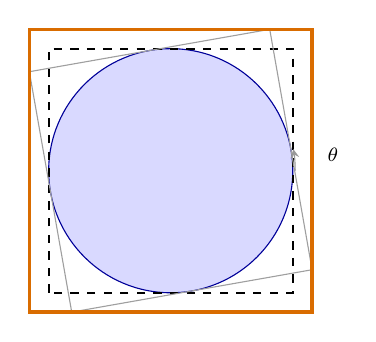
\begin{tikzpicture}[scale=1.55]
  \fill[blue!15] (0,0) circle (1);
  \draw[blue!60!black] (0,0) circle (1);
  \draw[dashed,thick] (-1,-1) rectangle (1,1);
  \begin{scope}[rotate=10]
    \draw[gray!75] (-1,-1) rectangle (1,1);
  \end{scope}
  \draw[very thick,orange!85!black] (-1.1585,-1.1585) rectangle (1.1585,1.1585);
  \draw[->,>=stealth,gray!80] (1.02,0) arc (0:10:1.02);
  \node[font=\scriptsize] at (1.33,0.13) {$\theta$};
\end{tikzpicture}
\end{minipage}\hfill
\begin{minipage}[b]{0.53\textwidth}
\centering
\footnotesize
\begin{tabular}{@{}rrrr@{}}
\toprule
$\theta$ & Kantenlänge & Fläche & $\mathrm{IoU}(\theta)$ \\
\midrule
 $2^\circ$ & $+3{,}4\,\%$ & $+7{,}0\,\%$ & 0{,}935 \\
 $5^\circ$ & $+8{,}4\,\%$ & $+17{,}6\,\%$ & 0{,}850 \\
$10^\circ$ & $+15{,}8\,\%$ & $+34{,}2\,\%$ & 0{,}745 \\
$20^\circ$ & $+28{,}2\,\%$ & $+64{,}4\,\%$ & 0{,}608 \\
$45^\circ$ & $+41{,}4\,\%$ & $+100{,}0\,\%$ & 0{,}500 \\
\bottomrule
\end{tabular}
\end{minipage}
\caption[Boxaufblähung unter Bildrotation]{Bildrotation als Quelle von
Labelrauschen. Links: Ein rotationssymmetrisches Objekt (Kreis) behält unter
Rotation dieselbe korrekte Box (schwarz gestrichelt); die mitgedrehte Box
(grau) und ihre achsparallele Hülle (orange) sind jedoch größer. Rechts: Werte nach
Gleichung~\eqref{eq:boxrot} und \eqref{eq:ioutheta} für eine quadratische Box.
Bereits bei $10^\circ$ liegt die Überlappung zwischen Label und Wahrheit bei
0,745 und damit unterhalb der Schwelle, ab der die Metrik \mAPseven{} einen
Treffer zählt.}
\label{abb:boxrotation}
\end{figure}

Abbildung~\ref{abb:boxrotation} zeigt: Schon eine Rotation um $10^\circ$ senkt
die Übereinstimmung zwischen Label und Wahrheit auf 0,745 -- ein Wert, der in
der Bewertung nach \mAPseven{} bereits als Fehltreffer gilt. Für ein Objekt von
25\px{} Durchmesser wächst die Boxkantenlänge dabei um rund 4\px{}. Das ist
kein akademischer Randeffekt, sondern systematisches Rauschen im Zielsignal der
Boxregression, dem das Netz nicht entkommen kann. Die Konsequenz für den Entwurf:
Bildrotation, Scherung und Perspektive dürfen \emph{nicht} als globale
Trainingszeit-Augmentierung eingesetzt werden, wenn dieselbe Variation auch
label-exakt erzeugt werden kann. Genau das leistet ein Generator, der die Box
nach der Transformation aus der transformierten Alphamaske neu bestimmt
(Abschnitt~\ref{sec:instanzgeometrie}).

\subsection{Kleine Objekte: die IoU-Metrik wird zur Auflösungsmessung}
\label{sec:ioukleinobjekt}

Der zweite Effekt betrifft die Empfindlichkeit der Bewertung. Verschiebt man
eine quadratische Box der Kantenlänge $d$ um $\delta$ Pixel in einer Achse, so
gilt
\begin{equation}
\mathrm{IoU} \;=\; \frac{(d-\delta)\,d}{2d^2 - (d-\delta)\,d}
\;=\; \frac{1 - \delta/d}{1 + \delta/d}.
\label{eq:ioushift}
\end{equation}
Der Fehler wirkt also ausschließlich über das \emph{Verhältnis} $\delta/d$. Für
ein 20\px{}-Objekt kostet ein Boxfehler von 2\px{} bereits 0,18 IoU
($\mathrm{IoU} = 0{,}818$), bei diagonaler Verschiebung um jeweils 2\px{} sogar
0,32 ($\mathrm{IoU} = 0{,}681$). Für ein 200\px{}-Objekt wäre derselbe absolute
Fehler mit 0,02 IoU praktisch unsichtbar.

Daraus folgen zwei Dinge. Erstens ist \mAPall{} bei Objekten dieser Größe mehr
ein Maß für die Pixelauflösung als für die Detektionsqualität -- ein Befund, der
in Abschnitt~\ref{sec:hauptergebnis} empirisch bestätigt wird. Zweitens ist
jedes Prozent Labelrauschen in der Boxposition bei kleinen Objekten teurer als
bei großen; die Anforderung an die Labelexaktheit der Augmentierung steigt also
mit sinkender Objektgröße.

\subsection{Skalierung und effektive Objektgröße}
\label{sec:effektivgroesse}

Detektoren verarbeiten Bilder in einer festen Netzeingangsgröße $M$
(\code{imgsz}). Ein Bild mit längster Kante $N$ wird dazu um den Faktor $M/N$
skaliert. Ein Objekt mit Durchmesser $d$ im Original erreicht das Netz damit mit
\begin{equation}
d_{\text{eff}} \;=\; d \cdot \frac{M}{N}.
\label{eq:deff}
\end{equation}
Damit es auf der feinsten Detektionsebene mit Gesamtschrittweite $S$ überhaupt
mehr als eine Gitterzelle belegt, muss $d_{\text{eff}} > S$ gelten. Für
$S = 8$, ein Bild mit $N = 2459$ und ein Objekt von $d = 27$\px{} ergibt
Gleichung~\eqref{eq:deff} bei $M = 640$ lediglich $d_{\text{eff}} = 7{,}0$\px{}
-- unterhalb der Grenze. Dies ist die quantitative Fassung des in
Abschnitt~\ref{sec:schwaechen} beschriebenen Auflösungsproblems und die
Erklärung für den in Abschnitt~\ref{sec:imgsz} gemessenen, dominanten Effekt der
Inferenzauflösung.

Für die Augmentierung folgt daraus eine wichtige Randbedingung: Die
Größenverteilung der Objekte in den Trainingsdaten und die effektive
Größenverteilung zur Inferenzzeit müssen übereinstimmen. Eine
Trainingszeit-Skalierung, die Objekte unter $S$ schrumpfen lässt, erzeugt Labels
ohne auflösbares Objekt -- also wiederum Labelrauschen. \textcite{kisantal2019}
adressieren dieselbe Problematik von der anderen Seite, indem sie kleine Objekte
im Trainingsdatensatz gezielt überabtasten und mehrfach einkopieren.

\subsection{Mehrbildverfahren bei der Detektion}

Mosaic \parencite{bochkovskiy2020} fügt vier Trainingsbilder zu einem zusammen.
Es ist bei der Detektion aus drei Gründen wirksam: Es erhöht die Objektzahl pro
Iteration, es bringt Objekte systematisch an Kachelränder (was angeschnittene
Objekte simuliert) und es kombiniert verschiedene Hintergründe in einem Bild.
Die Boxen bleiben dabei exakt, da nur beschnitten und verschoben wird. Zu
beachten ist die Kehrseite: Mosaic erzeugt eine Bildstatistik -- vier
zusammengesetzte Kacheln --, die es zur Inferenzzeit nie gibt. Die in der
YOLO-Werkzeugkette übliche Gegenmaßnahme ist das Abschalten von Mosaic in den
letzten Trainingsepochen (\code{close\_mosaic}), damit das Modell auf der echten
Bildstatistik ausklingt \parencite{ultralyticsdocs}.

Für mixup \parencite{zhang2018mixup} und CutMix \parencite{yun2019cutmix} gilt
das nicht in gleicher Weise. Beide überlagern Bildinhalte, während die Labels
beider Quellbilder bestehen bleiben. Bei der Klassifikation ist das durch die
Mischung des Zielvektors konsistent begründbar; bei der Detektion entstehen
halbtransparente \enquote{Geisterobjekte} mit vollem Boxlabel. Bei dicht
gepackten Kleinobjekten -- 20\px{} groß, im Median einen Durchmesser
voneinander entfernt -- ist der Anteil solcher Geisterobjekte hoch, und der
resultierende Labelkonflikt wirkt wie Rauschen.

\section{Automatisierte Suche von Augmentierungsstrategien}
\label{sec:autoaug}

Da $p(t)$ aus Gleichung~\eqref{eq:erm-aug} ein Hyperparameter ist, liegt es nahe,
sie zu optimieren. AutoAugment \parencite{cubuk2019} sucht mit
Reinforcement Learning nach Sequenzen von Transformationen und deren Stärken;
RandAugment \parencite{cubuk2020} reduziert den Suchraum auf zwei Parameter
(Anzahl und Stärke der Operationen) und erreicht damit vergleichbare Ergebnisse
bei drastisch geringeren Suchkosten; TrivialAugment \parencite{mueller2021}
verzichtet ganz auf die Suche und zieht Operation und Stärke gleichverteilt.
\textcite{zoph2020} übertragen den Ansatz auf die Detektion und finden
Strategien, die boxbezogene Operationen enthalten.

Für die vorliegende Arbeit sind diese Verfahren aus zwei Gründen nicht
anwendbar. Erstens setzt jede Suche einen Bewertungssplit voraus, auf dem die
Kandidatenstrategien verglichen werden; hier existiert genau \emph{ein} reales
Validierungsbild mit 88 Objekten, und dessen Metrikstreuung ist größer als die
zu erwartenden Unterschiede zwischen Strategien
(Abschnitt~\ref{sec:bootstrap}). Eine Suche darauf würde die Strategie an ein
Einzelbild anpassen. Zweitens -- und grundsätzlicher -- optimieren diese
Verfahren die Stärke \emph{gegebener} Operationen; die hier wesentlichen
Entscheidungen betreffen jedoch die Frage, welche Operationen überhaupt
physikalisch zulässig sind (etwa: darf ein Rohrende ohne Schaft existieren?).
Diese Frage ist eine Modellierungsfrage und keine Suchfrage.

\section{Grenzen und Risiken}
\label{sec:auggrenzen}

\absatz{Labelrauschen.} Behandelt in Abschnitt~\ref{sec:boxrotation}: Jede
Transformation, deren Labeltransformation nur approximativ bekannt ist, erzeugt
Rauschen im Zielsignal. Bei kleinen Objekten ist dieses Rauschen besonders
teuer.

\absatz{Verteilungsverschiebung.} Augmentierung verschiebt die
Trainingsverteilung gegenüber der Testverteilung, wenn sie Bilder erzeugt, die
zur Inferenzzeit nicht auftreten. Das Beispiel Mosaic wurde genannt; allgemeiner
gilt, dass eine zu breite Augmentierung Kapazität auf Regionen des Eingaberaums
lenkt, die praktisch irrelevant sind. Die Wirkung ist nicht monoton: Mehr
Augmentierung ist nicht besser, sondern hat ein Optimum, das von der
Datensatzgröße abhängt \parencite{cubuk2020}.

\absatz{Verwässerung diskriminativer Merkmale.} Wird ein Merkmal, das die Klasse
tatsächlich definiert, durch Augmentierung wegvariiert, sinkt die Trennschärfe.
Im vorliegenden Fall betrifft dies die Rundheit der Profile: Eine zu hohe Rate
an Verformungen (\enquote{Dellen}) würde die Kreisform als Merkmal entwerten und
Falschpositive auf beliebigen dunklen Flecken erzeugen. Solche Anteile sind
daher nach oben zu begrenzen und, wenn keine Messung vorliegt, ausdrücklich als
Annahme zu kennzeichnen.

\absatz{Nicht messbarer Nutzen.} Der Effekt einer einzelnen Transformation ist
nur über eine Ablation nachweisbar -- also über ein vollständiges
Trainings- und Bewertungsdurchlauf-Paar. Bei 25 Transformationen sind
vollständige Leave-one-out-Ablationen mit dem Rechenbudget einer Abschlussarbeit
nicht darstellbar. Ein ehrlicher Bericht muss daher unterscheiden zwischen
\emph{begründeten} und \emph{belegten} Entscheidungen. Diese Unterscheidung wird
in Kapitel~\ref{kap:diskussion} explizit gezogen.

\section{Grenzfall: rein synthetische Trainingsdaten}
\label{sec:augsynthese}

\subsection{Copy-Paste-Synthese und Domänenrandomisierung}

Wird die Augmentierung so weit getrieben, dass sie die Trainingsdaten nicht
erweitert, sondern erzeugt, entsteht synthetische Datengenerierung. Zwei
Traditionslinien sind hier relevant.

Die erste ist \textbf{Copy-Paste-Synthese}: Freigestellte Objekte werden in reale
Hintergrundbilder eingesetzt. \textcite{dwibedi2017} zeigen, dass dies für
Instanzdetektion überraschend gut funktioniert, und identifizieren als
entscheidenden Faktor nicht die globale Bildplausibilität, sondern die lokale
\emph{Grenzflächenqualität}: Wichtig ist, dass an der Objektkante keine
verräterischen Artefakte entstehen. \textcite{georgakis2017} verfolgen denselben
Ansatz für Innenraumszenen und betonen zusätzlich die Bedeutung
maßstabsgerechten Einsetzens: Objekte müssen an Positionen und in Größen
erscheinen, die mit der Szenengeometrie verträglich sind -- ein Argument, das im
vorliegenden Fall der Kopplung von Objektgröße und Rohrdurchmesser des
Hintergrunds entspricht (Abschnitt~\ref{sec:hintergrundstufe}).
\textcite{dvornik2018} widersprechen
teilweise und zeigen, dass auch der Kontext eine Rolle spielt -- Objekte an
kontextuell unmöglichen Orten schaden. \textcite{ghiasi2021} zeigen für die
Instanzsegmentierung, dass selbst sehr einfaches, kontextfreies Copy-Paste ein
starker Augmentierer ist, sofern Skalenvariation vorhanden ist. Diese
Arbeiten zusammen ergeben die Entwurfsregel, die auch hier gilt:
\emph{Grenzfläche und Skala sind kritisch, Kontext ist wichtig, globale
Bildästhetik ist nachrangig.}

Die zweite Linie ist \textbf{Domain Randomization}
\parencite{tobin2017,tremblay2018}. Ihre Grundidee ist gegenläufig: Statt
Realismus anzustreben, wird so viel Variation erzeugt, dass die reale Welt dem
Netz nur als eine weitere Variation erscheint. \textcite{prakash2019} verbinden
beides zur \emph{strukturierten} Domänenrandomisierung, bei der die Variation
innerhalb physikalisch plausibler Grenzen erfolgt.
\textcite{hinterstoisser2018} zeigen zusätzlich, dass vortrainierte
Merkmalsextraktoren den Übergang deutlich erleichtern, weil die
domänenunabhängigen Low-Level-Filter nicht aus synthetischen Daten gelernt
werden müssen -- ein Argument, das die Verwendung COCO-vortrainierter Gewichte
in dieser Arbeit stützt (vgl.\ \cite{yosinski2014}). Ein Überblick über den
gesamten Bereich findet sich bei \textcite{nikolenko2021}.

Die hier verfolgte Pipeline liegt zwischen beiden Linien: Sie randomisiert
breit, aber ausschließlich innerhalb physikalisch möglicher Konfigurationen --
und sie nutzt als Hintergründe keine gerenderten Szenen, sondern
\emph{Aufnahmen der Zieldomäne selbst}.

\subsection{Warum der Übergang misslingt, wenn er misslingt}

Der Nutzen synthetischer Daten hängt daran, wie ähnlich die erzeugte Verteilung
$D_S$ der Zielverteilung $D_T$ ist. \textcite{bendavid2010} geben dafür eine
obere Schranke des Zielfehlers an: Für eine Hypothese $h$ aus einer
Hypothesenklasse $\mathcal{H}$ gilt
\begin{equation}
\varepsilon_T(h) \;\leq\; \varepsilon_S(h)
\;+\; d_{\mathcal{H}\Delta\mathcal{H}}(D_S, D_T)
\;+\; \lambda,
\label{eq:bendavid}
\end{equation}
wobei $\varepsilon_S$ der Fehler auf der Quellverteilung,
$d_{\mathcal{H}\Delta\mathcal{H}}$ eine Divergenz zwischen den beiden
Eingabeverteilungen und $\lambda$ der Fehler der besten gemeinsamen Hypothese
ist. Gleichung~\eqref{eq:bendavid} ist für den Pipelineentwurf nützlich, weil sie
die möglichen Angriffspunkte vollständig auflistet:

\begin{enumerate}[label=(\roman*)]
  \item \textbf{$\varepsilon_S$ klein halten} -- also überhaupt erst lernbare,
  korrekt gelabelte synthetische Daten erzeugen. Hierher gehört die exakte
  Sichtbarkeitsrechnung (Abschnitt~\ref{sec:sichtbarkeit}): Labels für praktisch
  unsichtbare Objekte erhöhen $\varepsilon_S$ unvermeidbar.
  \item \textbf{$d_{\mathcal{H}\Delta\mathcal{H}}$ klein halten} -- die
  Verteilungen einander annähern. Das ist der Zweck aller Kalibrierungen an
  Realmessungen (Objektgröße, Seitenverhältnis, Nachbarschaftsabstände) und aller
  Maßnahmen zum Einbettungsrealismus (Farb-, Unschärfe-, Rauschangleich,
  JPEG-Requantisierung). Wichtig ist die Struktur des Terms: Die Divergenz wird
  über die Hypothesenklasse gemessen, also über die Funktionen, die das Netz
  überhaupt bilden kann. Ein Unterschied, den ein CNN leicht erkennen kann --
  eine achsparallele Naht, ein konstanter Farbversatz --, trägt daher weit stärker
  zu $d_{\mathcal{H}\Delta\mathcal{H}}$ bei als ein Unterschied, für den es keine
  einfache Entscheidungsfunktion gibt.
  \item \textbf{$\lambda$ klein halten} -- sicherstellen, dass eine Hypothese
  existiert, die auf beiden Verteilungen gut ist. Praktisch heißt das: Die
  \emph{Labeldefinition} muss in Quelle und Ziel identisch sein. Deshalb erzeugt
  die Pipeline modale Boxen (den sichtbaren Umriss) und keine amodalen, und
  deshalb verwirft sie Labels nach denselben Regeln, nach denen die Realbilder
  annotiert wurden (Abschnitt~\ref{sec:sichtbarkeit}).
\end{enumerate}

\subsection{Shortcut Learning als konkrete Fehlerquelle}
\label{sec:shortcut}

Punkt~(ii) verdient eine eigene Betrachtung, weil er die Hauptfehlerquelle der
Copy-Paste-Synthese darstellt. \textcite{geirhos2020} beschreiben unter dem
Begriff \emph{Shortcut Learning} das allgemeine Phänomen, dass neuronale Netze
bevorzugt jene Merkmale nutzen, die auf den Trainingsdaten am einfachsten zum
Ziel führen -- auch wenn diese Merkmale mit der eigentlichen Aufgabe nichts zu
tun haben und außerhalb der Trainingsverteilung nicht mehr gelten.
\textcite{torralba2011} zeigen mit ihrem \enquote{Name that dataset}-Experiment,
dass schon gewöhnliche Bilddatensätze an solchen Merkmalen erkennbar sind.

Bei eingeklebten Objekten sind die Abkürzungen benennbar. Die
Bildforensik untersucht seit Langem genau diese Signaturen, um Bildmontagen
nachzuweisen \parencite{farid2009} -- was hier als Katalog der zu schließenden
Lücken gelesen werden kann:

\begin{enumerate}[label=\textbf{S\arabic*.},leftmargin=2.6em]
  \item \textbf{Geometrische Naht.} Ein rechteckiger Ausschnitt hinterlässt eine
  achsparallele Kante. Sie ist für ein CNN mit $3\times3$-Kerneln trivial
  detektierbar und daher die perfekte Abkürzung. Gegenmaßnahme: echtes
  Freistellen mit weicher Alphamaske (Abschnitt~\ref{sec:matting}).
  \item \textbf{Farb- und Helligkeitsversatz.} Objekt und Hintergrund stammen aus
  Aufnahmen mit unterschiedlichem Weißabgleich und Belichtungsniveau. Der
  resultierende konstante Versatz ist ein global gültiges Merkmal.
  Gegenmaßnahme: partieller Statistikangleich im Stil des Farbtransfers von
  \textcite{reinhard2001}; das Forschungsfeld der \emph{Image Harmonization}
  \parencite{tsai2017} behandelt genau dieses Problem.
  \item \textbf{Schärfe- und Auflösungsversatz.} Ein skaliertes Objekt hat eine
  andere Modulationsübertragung als das Zielbild;
  \textcite{popescu2005} weisen Montagen genau über solche Resampling-Spuren
  nach. Aliasing durch ungeeignete Interpolation erzeugt zudem
  Hochfrequenzmuster, gegen die CNNs bekanntermaßen empfindlich sind
  \parencite{zhangr2019}. Gegenmaßnahme: flächentreue Verkleinerung und
  gezielter Unschärfeangleich.
  \item \textbf{Rauschversatz.} Beim Verkleinern sinkt das Sensorrauschen eines
  Ausschnitts; der eingeklebte Bereich ist dann messbar \enquote{sauberer} als
  seine Umgebung. Sensorrauschen ist so charakteristisch, dass es zur
  Kameraidentifikation genutzt wird \parencite{lukas2006}. Gegenmaßnahme:
  Rauschangleich mit einer lokal geschätzten Amplitude
  \parencite{immerkaer1996}.
  \item \textbf{Kompressionsversatz.} Der Hintergrund war bereits einmal
  JPEG-komprimiert, die eingefügten Pixel nicht; die DCT-Blockstatistik
  unterscheidet sich \parencite{wallace1992jpeg,farid2009}. Gegenmaßnahme:
  erneute JPEG-Requantisierung des \emph{Gesamtbildes}.
  \item \textbf{Fehlende Szeneninteraktion.} Ohne Kontaktschatten und ohne
  plausible Verdeckung \enquote{schwebt} ein eingefügtes Objekt sichtbar. Dies
  ist derselbe Hinweis, den auch menschliche Betrachter nutzen. Gegenmaßnahme:
  Schlagschatten und physikalisch motivierte Verdeckung.
\end{enumerate}

Der entscheidende Punkt ist, dass bei Copy-Paste-Synthese \emph{nicht zu wenig
Variation} die dominante Fehlerquelle ist, sondern \emph{systematische}
Unterschiede zwischen eingefügten und originalen Pixeln. Variation lässt sich
durch mehr Zufall erzeugen; ein systematischer Versatz bleibt bei beliebig viel
Zufall bestehen und wird vom Netz zuverlässig gefunden.

\section{Anforderungen an die Pipeline}
\label{sec:anforderungen}

Aus den vorstehenden Abschnitten ergeben sich sechs Anforderungen, an denen sich
der Entwurf in Kapitel~\ref{kap:pipeline} messen lässt. Sie werden dort jeweils
referenziert.

\begin{description}[leftmargin=3.2em,style=nextline]
  \item[A1 -- Labelexaktheit] Jede Transformation muss eine exakt bekannte
  Labeltransformation besitzen. Transformationen, die achsparallele Boxen
  aufblähen, sind im Bild verboten und stattdessen pro Instanz mit
  Neuberechnung der Box auszuführen (Abschnitt~\ref{sec:boxrotation}).
  \item[A2 -- Kalibrierte Skala] Die Größenverteilung der erzeugten Objekte muss
  der real gemessenen entsprechen, und die Trainingsauflösung muss so gewählt
  sein, dass die Objekte oberhalb der Auflösungsgrenze des feinsten
  Detektionskopfes liegen (Abschnitt~\ref{sec:effektivgroesse}).
  \item[A3 -- Physikalische Zulässigkeit] Erzeugt werden nur Konfigurationen,
  die real auftreten können. Invarianzen werden nur dort antrainiert, wo sie
  tatsächlich gelten (Abschnitt~\ref{sec:augformal}).
  \item[A4 -- Geschlossene Abkürzungen] Für jede der Signaturen S1--S6 aus
  Abschnitt~\ref{sec:shortcut} muss eine Gegenmaßnahme existieren.
  \item[A5 -- Identische Labeldefinition] Die Regeln, nach denen ein Objekt ein
  Label erhält, müssen mit den Regeln der Handannotation der Realbilder
  übereinstimmen (Term $\lambda$ in Gleichung~\eqref{eq:bendavid}).
  \item[A6 -- Dokumentierte Verteilung] Für jede Transformation sind
  Parameterbereich \emph{und} tatsächlicher Anteil im erzeugten Datensatz
  anzugeben; Werte ohne Messbelege sind als Annahme zu kennzeichnen
  (Abschnitt~\ref{sec:augformal}).
\end{description}
